\subsection{API REST}

\begin{frame}{Nos réalisations}{API REST}

\textbf{Les routes de l'application}

\begin{table}
    \begin{tabulary}{\textwidth}{|C C C|}
        \hline
        \rowcolor{primaryLight}\color{background}{Méthode HTTP} & \color{background}{URI} & \color{background}{Paramètres}\\
        \hline
	    GET & api/subnet & \\
	    POST & api/subnet?<parametres> & ip, next\_hop, communities \\
	    PUT & api/subnet?<parametres> & TOUS \\
	    PATCH & api/subnet?<parametres> & id, is\_activated \\
	    DELETE & api/subnet?<parametre> & id \\
	    \hline
	\end{tabulary}
\end{table}

\end{frame}

\begin{frame}[fragile]{Nos réalisations}{Format JSON}
    \begin{minipage}{0.3\textwidth}
        \begin{minted}{js}
            [
              {
                "communities": [
                  "50:52"
                ], 
                "created_at": "2019-02-18T17:38:47", 
                "id": "5c6adf97f16dda55fcc79151", 
                "ip": "192.168.0.1", 
                "is_activated": true, 
                "last_activation": "2019-02-19T14:52:21", 
                "modified_at": "2019-02-19T14:52:21", 
                "next_hop": "1.1.1.1"
              }
          ]
        \end{minted}
    \end{minipage}
\end{frame}

\begin{frame}{Nos réalisations}{Architecture de l'API REST}
    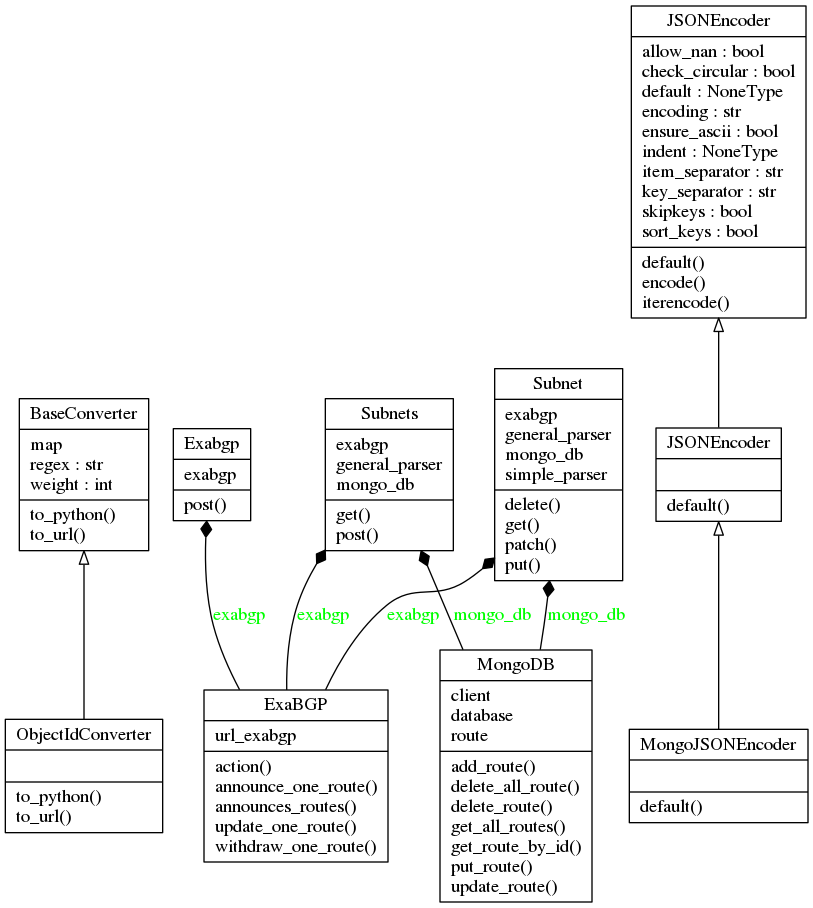
\includegraphics[width=\textwidth, height=0.7\textwidth]{classes_backend.png}
\end{frame}